% Chapter 4
% Roberto Masocco <robmasocco@gmail.com>
% October 8, 2021

\chapter[Controllori e middleware]{Controllori e middleware}
\label{chap:Chapter4} 
\doublespacing
\fontsize{12}{12}\selectfont
\newsection{Premessa}
\indent Nel Capitolo \ref{chap:Chapter3} è stata discussa l'implementazione di un'architettura di controllo basata sul middleware ROS 2. Su tale architettura sono state realizzate le logiche di controllo e supervisione di livello medio-alto del drone autonomo presentato come caso di studio. L'obiettivo di questo capitolo è presentare uno studio preliminare delle possibilità di tale architettura in contesti di più basso livello, relativi ai sistemi di controllo veloci. Verrà dunque esaminato un problema di controllo relativo allo stesso caso di studio precedente, e verranno discusse delle sue soluzioni realizzate come moduli dell'architettura illustrata nel capitolo precedente, testate usando il modello del drone simulato in Gazebo.

\newsection{Problema di controllo}
\indent Il precision landing è una fase critica della missione: dal suo corretto svolgimento dipende l'assegnazione del punteggio relativo alla piazzola su cui lo si esegue. Qualunque disturbo presente in fase di allineamento e discesa, se non correttamente reiezionato, può compromettere la stabilità del volo e dunque la precisione dell'atterraggio sul target.\\
Il problema di controllo che verrà ora studiato è quello del precision landing in presenza di vento. Quest'ultimo è inteso come un disturbo costante di ampiezza e segno non noti a priori, che va a sommarsi alla velocità assunta dal drone mediante il suo sistema di controllo veloce illustrato precedentemente. Si assume inoltre che, per effettuare la procedura con la massima precisione possibile, il drone sia controllato in velocità lineare mediante invio di setpoint appositi, calcolati da un opportuno controllore il cui ingresso sia un segnale d'errore di posizionamento rispetto al target, espresso in metri e campionato dalla camera inferiore a 20 Hz grazie ad uno dei moduli precedentemente descritti. Tale soluzione si configura dunque come un'alternativa rispetto a quella presentata nel Capitolo \ref{chap:Chapter3} e implementata nel modulo Land Corrector, che era basata su una correzione del posizionamento richiesta direttamente al controllo di posizione di PX4. Per semplicità verranno controllati separatamente i posizionamenti lungo gli assi X ed Y del sistema di riferimento solidale al suolo, mentre la quota verrà progressivamente abbassata fintantoché l'allineamento sarà corretto secondo la stessa logica del modulo originale, e sempre mediante un controllo in velocità proporzionale alla differenza tra la quota corrente ed il nuovo riferimento.

\newsection{Identificazione del sistema da controllare}
\indent Il problema descritto poc'anzi richiede un'analisi preliminare del sistema da porre sotto controllo: si tratta infatti di una situazione non-standard. Si vuole, in sintesi, controllare il drone, già sotto il controllo stabilizzante del Pixhawk, impostando un riferimento di velocità da fargli inseguire, mediante delle azioni di controllo realizzate dai motori che sono però calcolate da PX4 e supposte ignote. Nonostante l'ipotesi semplificativa di separare il controllo sui due assi, è necessario identificare due diversi sistemi, che esprimano il modo in cui il drone stabilizzato insegue riferimenti di velocità su ciascun asse. Tali sistemi saranno chiaramente nonlineari nella realtà, ma ai fini di questo lavoro è stata giudicata sufficiente una loro approssimazione con modelli lineari di ordine opportuno.\\
La fase di raccolta dati è stata eseguita su Gazebo, impiegando il modulo Flight Control per controllare il drone e definendo delle routine di test per ciascun asse che consistevano nell'invio di diversi setpoint di velocità da inseguire, implementate come script di shell. Durante i voli di prova sono stati registrati tramite bagging i dati di input/output su cui lavorare, nella forma di setpoint correnti e velocità misurate da EKF2 ad ogni istante: i primi inviati dal nodo flight\_controller a 20 Hz sul topic /TrajectorySetpoint e le seconde trasmesse da PX4 sul topic /VehicleOdometry a 100 Hz. Successivamente un nodo ROS 2 scritto ad-hoc ha consentito di ricampionare entrambi i segnali allo stesso rate dell'odometria, dunque 100 Hz, salvandoli infine tutti in un file CSV. I datasets così ottenuti sono mostrati nelle Figure \ref{fig:xdataset} e \ref{fig:ydataset}. Da essi si evince chiaramente come si tratti, in entrambi i casi, di sistemi approssimabili linearmente al primo ordine.\\
La procedura d'identificazione è stata eseguita con l'ausilio della System Identification Toolbox\footnote{https://it.mathworks.com/products/sysid.html} di MATLAB. Il Toolbox è stato impiegato in entrambi i casi per identificare la rappresentazione nello spazio di stato di un sistema lineare del primo ordine usando la \emph{Prediction Error Minimization}, da cui calcolare poi una funzione di trasferimento. I dataset sono stati divisi in due parti, usate rispettivamente per la stima e la validazione. Un confronto tra i modelli approssimati e quelli reali eseguito sui validation sets, unitamente agli intervalli di confidenza, è disponibile nelle Figure \ref{fig:xvalerr} e \ref{fig:yvalerr}, mentre le due funzioni di trasferimento ad essi corrispondenti sono:
\begin{subequations}
    \begin{align}
        W_x(s) &= \frac{1.1853}{s+1.2775}\\
        W_y(s) &= \frac{1.4219}{s+1.4350}.
    \end{align}
\end{subequations}

\begin{figure}
    \centering
    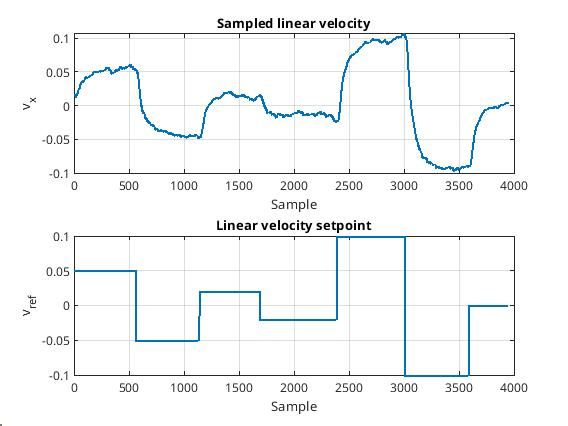
\includegraphics[width=0.8\textwidth]{figs/chapter4/xdataset.jpg}
    \caption{Dataset I/O relativo all'asse X.}
    \label{fig:xdataset}
\end{figure}

\begin{figure}
    \centering
    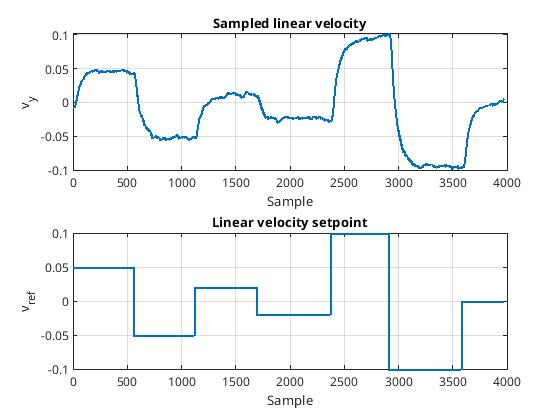
\includegraphics[width=0.8\textwidth]{figs/chapter4/ydataset.jpg}
    \caption{Dataset I/O relativo all'asse Y.}
    \label{fig:ydataset}
\end{figure}

\begin{figure}
    \centering
    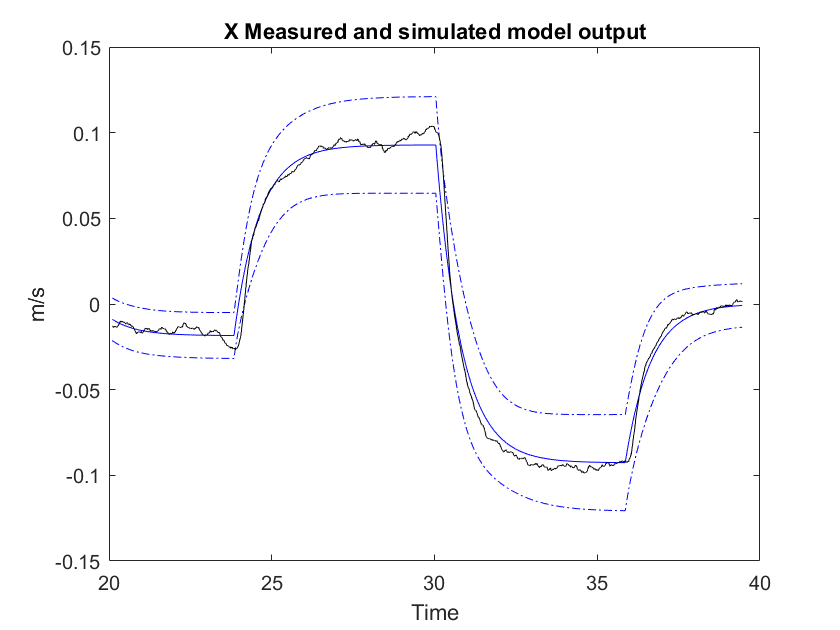
\includegraphics[width=0.7\textwidth]{figs/chapter4/valxtimeplot.png}
    \caption{Confronto tra l'output misurato e quello approssimato (in blu) sul validation set relativo all'asse X. In tratteggio i limiti dell'intervallo di confidenza.}
    \label{fig:xvalerr}
\end{figure}

\begin{figure}
    \centering
    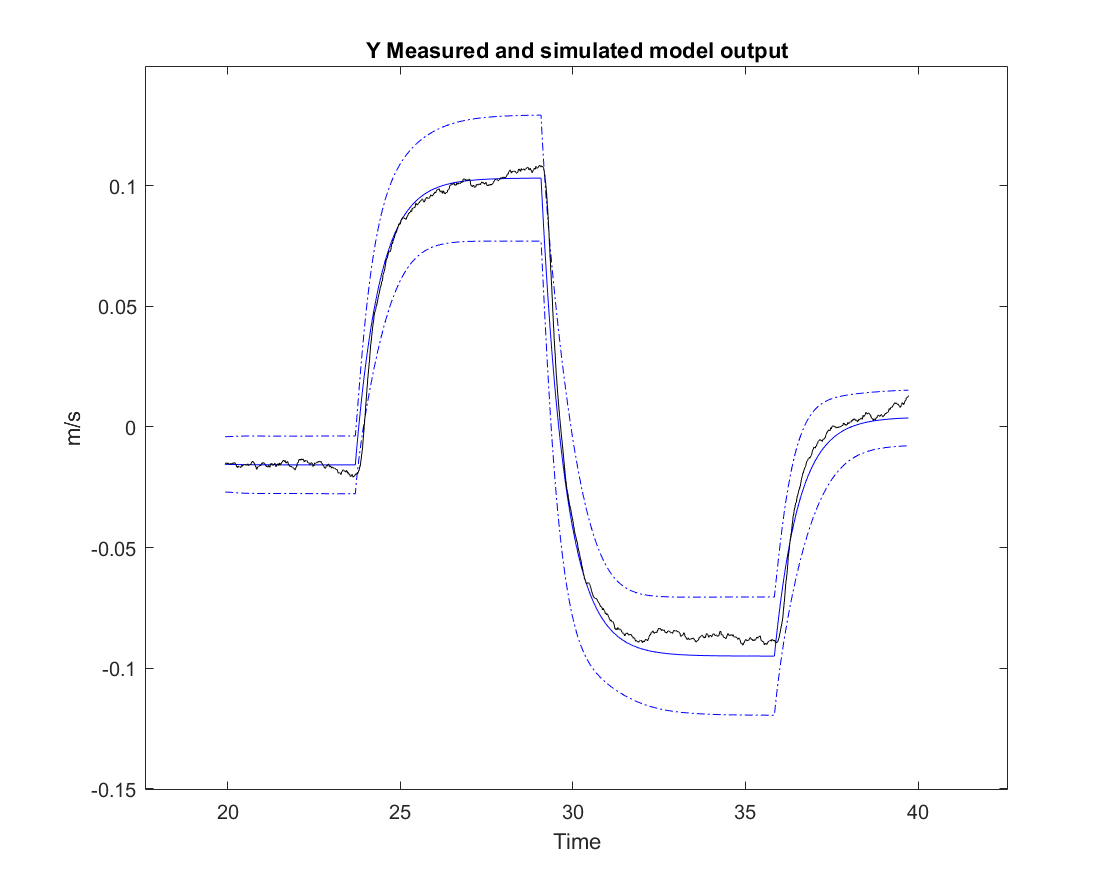
\includegraphics[width=0.7\textwidth]{figs/chapter4/valytimeplot.png}
    \caption{Confronto tra l'output misurato e quello approssimato (in blu) sul validation set relativo all'asse Y. In tratteggio i limiti dell'intervallo di confidenza.}
    \label{fig:yvalerr}
\end{figure}

\newsection{Design del controllore}
\indent prova
